% main.tex
\documentclass{article}

\usepackage[pdfauthor={CoderDojo Linz},
            pdftitle={Space Shooter}]
            {hyperref}

\newcommand{\footertitle}{Space Shooter}
% settings.tex
\usepackage[
    a4paper, 
    top=2cm,
    left=1cm,
    right=1cm,
    bottom=2cm
]{geometry}

\usepackage{fontspec}
\usepackage{graphicx}
\usepackage{hyperref}
\usepackage{fancyhdr}
\usepackage[ngerman]{babel}
\usepackage{wrapfig}
\usepackage{enumitem}
\usepackage{titlesec} 
\usepackage{ragged2e}
\usepackage{tcolorbox}
\usepackage{array}
\usepackage[table]{xcolor}
\usepackage{fontawesome5}

\setmainfont{Carlito}

% Fancyhdr setup
\fancypagestyle{defaultpagestyle}{
    \fancyhf{} % Clear all headers and footers
    \fancyhead[C]{
\includegraphics[width=5cm]{../../CoderDojo_Logo.png}} 
    \renewcommand{\headrulewidth}{0pt} % Remove header line
    \renewcommand{\footrulewidth}{0pt} % Remove footer line
    \fancyfoot[L]{\footertitle}
    \fancyfoot[R]{Seite \thepage} % Right footer with page number
}

\newcommand{\SectionDesign}[4]{
    \noindent
    \csname #1*\endcsname{\textcolor[HTML]{1E90FF}{\fontsize{#2pt}{#3pt}\selectfont #4}}
}

\newcommand{\TextAndImage}[5][{}]{
    \fontsize{11pt}{16pt}\selectfont
    \noindent
    \begin{minipage}[c]{#4\textwidth}
    \RaggedRight
    #2 % First parameter: text
    \end{minipage}
    \hfill
    \begin{minipage}[c]{#5\textwidth}
    \includegraphics[width=\textwidth, #1]{#3} % Second parameter: image file name
    \end{minipage}
}

\newcommand{\ImageAndText}[2]{
    \fontsize{16pt}{24pt}\selectfont
    \noindent
    \begin{minipage}[c]{0.65\textwidth}
        \includegraphics[width=\textwidth]{#1} % Second parameter: image file name
    \end{minipage}
    \hfill % Fills the space between the minipages
    \begin{minipage}[c]{0.25\textwidth}
        \centering
        #2 % First parameter: text
    \end{minipage}
}

\newcommand{\TextDesign}[1]{
    \fontsize{11pt}{16pt}\selectfont
    \noindent
    \RaggedRight
    #1 % First parameter: text
}
\graphicspath{{images/}}

\begin{document}
    \pagestyle{defaultpagestyle}

    \SectionDesign{section}{24}{24}{\textbf{Space Shooter}}
    \vspace{0.5cm}
     
    \ImageAndText{SpaceShooter.png}{
    \centering
    In dieser Übung schießt du mit deinem Raumschiff herabfallende Meteoriten ab bevor sie dein Raumschiff zerstören.
    }{0.65}{0.25}{16}{24}
    
    \vspace{1.5cm}
    \SectionDesign{subsection}{18}{24}{\textbf{Bühne und Figuren anlegen}}
    \vspace{0.5cm}

    \SectionDesign{subsubsection}{14}{24}{Spielfeld}
    \vspace{-1cm}
    
    \TextAndImage{
    \vspace{-0.5cm}
    Als erstes legst du fest, wie deine Bühne aussehen soll. Für dieses Spiel brauchst du das Weltall als Hintergrund. Wähle ein passendes Bild aus oder male selbst eines.}{Spielfeld.png}{0.45}{0.5}{11}{16}

    \vspace{1cm}
    \SectionDesign{subsubsection}{14}{24}{Figuren}
    \vspace{0.25cm}
    
    \ImageAndText{Figuren.png}{
    \vspace{-4.5cm}
    Als erste Figur brauchst du das Raumschiff. Du fügst es mit \textit{Figur wählen} ein.}{0.5}{0.45}{11}{16}

    \TextAndImage{
    \begin{adjustwidth}{5cm}{0cm}
    
        \RaggedLeft
        Die Figur muss aus zwei Kostümen bestehen: dem Raumschiff selbst und einem weiteren Kostüm, das angezeigt wird, wenn das Spiel vorbei ist. 
    
        \vspace{\baselineskip}
        Erstelle dazu ein eigenes Kostüm mit dem Text \textit{Game Over} oder male ein passendes Bild.
    \end{adjustwidth}
    }{FigurDesign.png}{0.6}{0.35}{11}{16}
    
    \vspace{1cm}
    
    \ImageAndText{FigurDesign2.png}{
    \vspace{-2cm}
    \begin{adjustwidth}{-14.5cm}{24cm}
    
        Die nächste Figur ist der Laserstrahl, der von der Rakete abgefeuert werden kann. Diesen kannst du dir selbst malen.
        
    \end{adjustwidth}
    }{0.2}{0.75}{11}{16}
    
    \vspace{1cm}

    \TextAndImage{
    \vspace{-2cm}
    \begin{adjustwidth}{8cm}{0cm}
        Und als letzte Figur brauchst du noch einen Meteoriten. Diesen kannst du dir selbst malen.
    \end{adjustwidth}
    }{FigurDesign3.png}{0.75}{0.2}{11}{16}

    \vspace{1cm}
    
    \ImageAndText{FigurDesign4.png}{
    \vspace{-1cm}
    \begin{adjustwidth}{-11cm}{12cm}
        Am Ende solltest du drei Figuren haben: Raumschiff, Laser und Meteor.
    \end{adjustwidth}
    }
    {0.4}{0.55}{11}{16}


    % NEW PAGE
    \newpage

    \TextAndImage{
    \vspace{-1cm}
    \SectionDesign{subsection}{18}{24}{\textbf{Variablen}}
    \vspace{0.5cm}
    
    Wir brauchen für den Space Shooter einige \textit{Variablen}: die Anzahl der Treffer, die Entstehungszeit von Meteoriten, deren Geschwindigkeit und einen Indikator, ob ein Meteorit getroffen wurde.

    \vspace{\baselineskip}
    \textbf{\textcolor[HTML]{1E90FF}{Achtung:} Die Variable getroffen gilt nur für die Figur “Meteorit”, alle anderen Variablen gelten \textit{für alle Figuren.}}}{Variablen.png}{0.4}{0.55}{11}{16}

    \vspace{1cm}
    
    \TextAndImage{
    \vspace{-9cm}
    \SectionDesign{subsection}{18}{24}{\textbf{Skripte für das Raumschiff}}
    \vspace{0.5cm}
    
    Das Raumschiff hat drei Aufgaben:

    \begin{itemize}
        \item Es muss erkennen, wann es von einem Meteoriten getroffen wurde und dann das Spiel beenden.
        \item Mit den Pfeiltasten kann es nach links und rechts bewegt werden.
        \item Mit den Tasten \textit{a} und \textit{d} kann es nach links und rechts gedreht werden.
    \end{itemize}
    }{SkriptRaumschiff.png}{0.5}{0.4}{11}{16}

    \vspace{-8cm}
    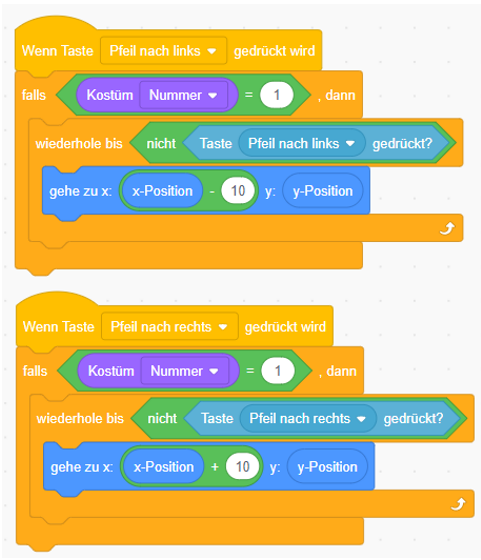
\includegraphics[width=8cm]{images/SkriptRaumschiff2.png}

    \vspace{0.25cm}
    \RaggedRight  
    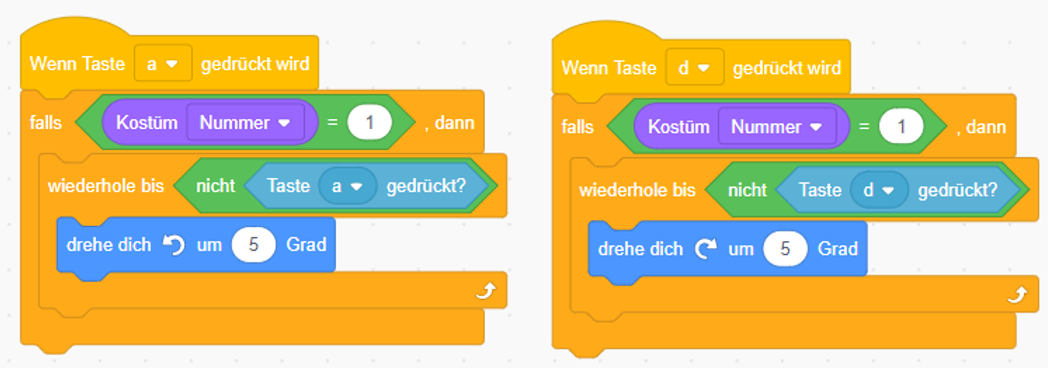
\includegraphics[width=16cm]{images/SkriptRaumschiff3.png}

    
    \vspace{0.5cm}
    \SectionDesign{subsection}{18}{24}{\textbf{Skripte für den Laser}}
    \vspace{0.25cm}
    
    \TextDesign{
    Jedes Mal, wenn die Leertaste gedrückt wird, muss ein neuer Laserstrahl erzeugt und abgefeuert werden. 
    }

    \vspace{0.5cm}
    \RaggedRight
    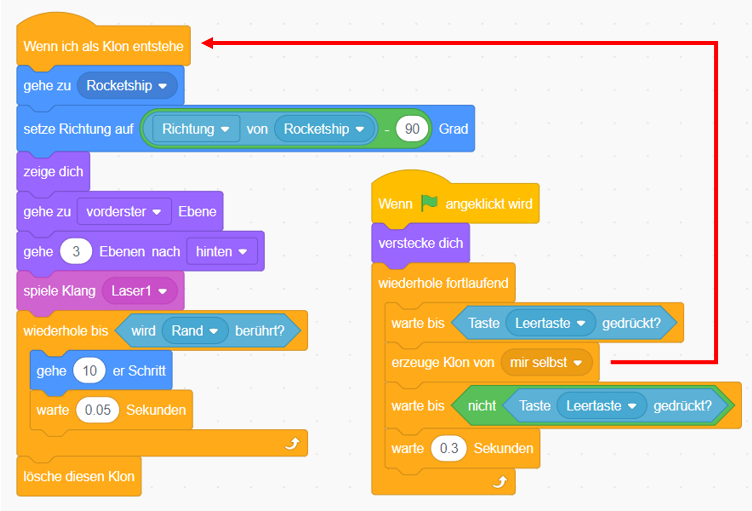
\includegraphics[width=16cm]{images/SkriptLaser.png}


    % NEW PAGE
    \newpage
    \SectionDesign{subsection}{18}{24}{\textbf{Skripte für den Meteoriten}}
    \vspace{0.5cm}
    
    \TextDesign{
    Für die Meteoriten brauchen wir eine Schleife, in der alle paar Sekunden ein neuer Meteorit erzeugt wird. Die Meteoriten müssen langsam nach unten fallen. Sie müssen verschwinden, wenn sie am unteren Bildschirmrand angekommen sind oder von einem Laser getroffen wurden.
    }

    \vspace{0.5cm}
    \RaggedRight  
    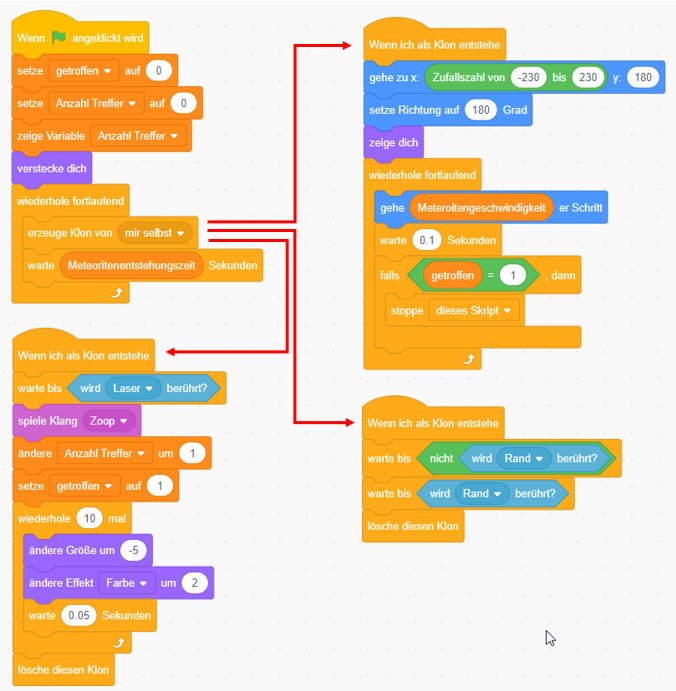
\includegraphics[width=16cm]{images/SkriptMeteoriten.png}
    
    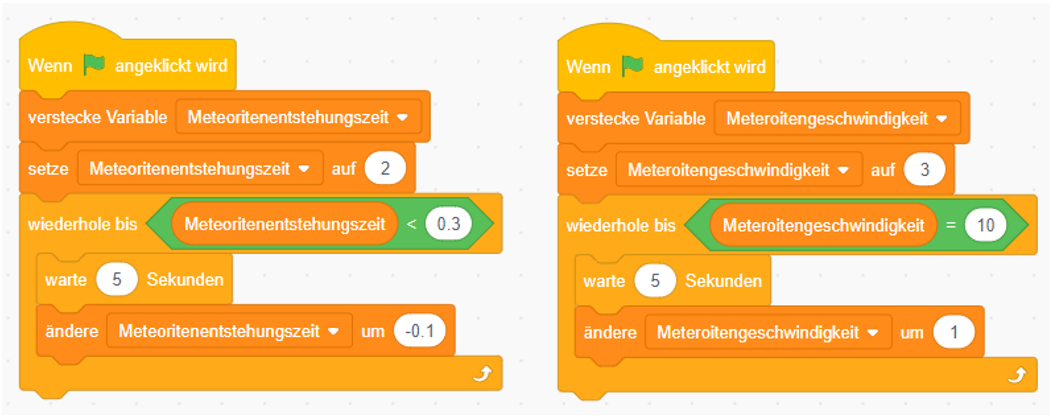
\includegraphics[width=16cm]{images/SkriptMeteoriten2.png}

    \vspace{0.5cm}
    \SectionDesign{subsection}{18}{24}{\textbf{Fertig!}}
    \vspace{0.5cm}
    
    \TextDesign{
    Gratuliere! Dein Spiel ist fertig. Probiere es gleich aus! Du kannst das fertige Projekt unter \href{https://meet.coderdojo.net/scratch-spaceshooter}{\textcolor{blue}{https://meet.coderdojo.net/\newline scratch-spaceshooter}} ausprobieren.
    }

    \vspace{0.5cm}
    \SectionDesign{subsection}{18}{24}{\textbf{Weitere Ideen}}
    
    \TextDesign{
    \begin{itemize}
        \item Füge verschiedene Arten von Meteoriten hinzu.
        \item Ändere den Hintergrund, je länger das Spiel läuft.
        \item Zeige den Feuerstrahl des Raumschiffs nur an, wenn es sich bewegt.
    \end{itemize}
    }
    
\end{document}

